\subsection{State-Machine-basierte Programmierung}\label{subsec:fsmprogrammierung}
\begin{quote}
    ''\textit{Have you tried turning it off and on again?}''  \\ -- Ein Jeder, der die Macht von \acp{FSM} verstanden hat.
\end{quote}

Bis zum jetzigen Zeitpunkt kann man den beschriebenen \ac{DBP}-Ansatz mit dem von SAM Labs (Kapitel \ref{subsubsec:samlabs}) vergleichen, auch mit seinen Problem (''Sequentiell contra Parallel'' und ''Signalpriorisierung''). Wie schon in den Problemen beschrieben, muss es Aktoren möglich sein mit parallel eintreffenden Signalen umgehen zu können, um Szenarien wie die in \hyperref[szenario2]{Szenario S\#2}  beschriebene Ampelschaltung und die in \hyperref[szenario3]{Szenario S\#3} beschriebene Vermeidung von Signalkonflikten zu ermöglichen.

Die einzige Möglichkeit für SAM Labs diesen Problemen aus dem Weg zu gehen ist es, sequentielle Logik mit der Datenfluss-Logik zu vermischen. Dies geschieht indem die Steuerungslogik der Aktoren, welche Entscheidungen über das Verhalten des Aktors treffen, auf der selben Ebene deklariert werden, wie die Logik, die Signale in eine nutzbare Form transformieren. In flowws wird einen anderen Weg gegangen. Es kommt eine Paradigma zum Steuern der Aktoren, welches weite Verbreitung in der IT und in \textit{Embedded Hardware} genießt: die \acl{FSM} (dt. ''endlicher Zustandsautomat'')

\begin{figure}[h]
  \centering
  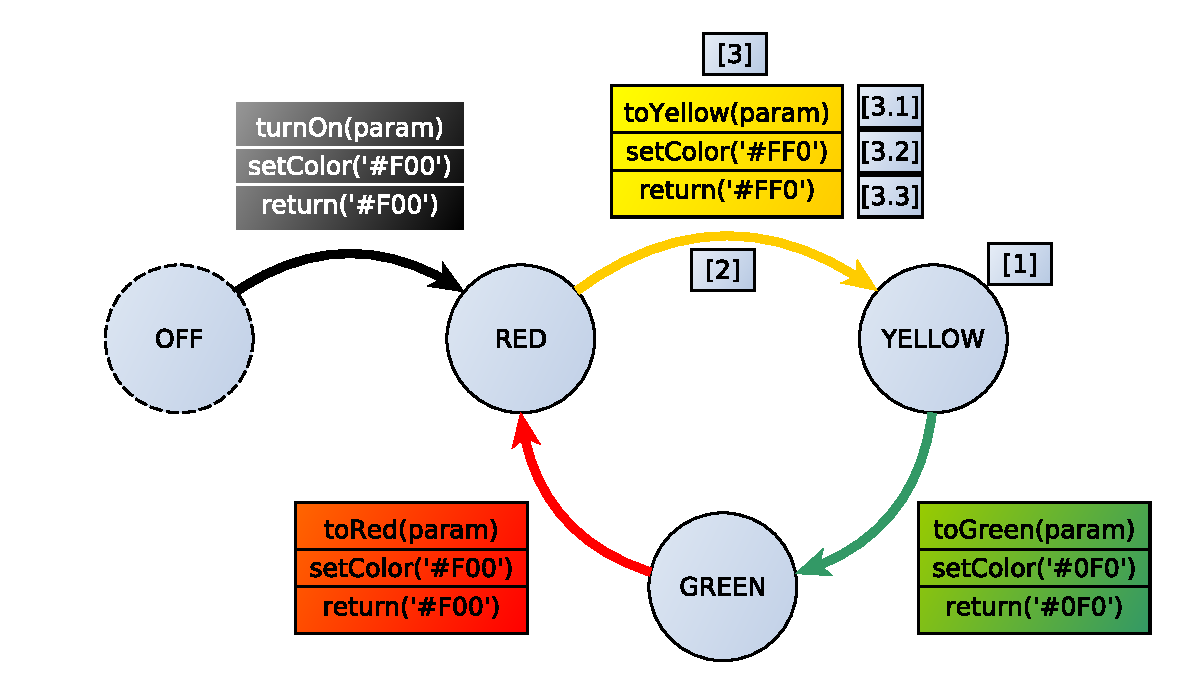
\includegraphics[width=0.85\textwidth]{bilder/chapter4/chapter4_2/beispielstatemachine.pdf}
  \caption{Die \ac{FSM} eines cBlocks mit LED-Aktor. Es existieren vier Zustände: OFF (Startzustand), RED, YELLOW, GREEN; und vier Übergänge: turnOn(), toYellow(), toGreen() und toRed(). Jeder der Übergänge verwendet in diesem Fall die setColor()-Funktion des LED-Aktors um die LED in der jeweils definierten Farbe wechseln. Jeder Übergang nimmt die Parameter (param) entgegen, was dem \textit{Payload} eines \textit{Events} entspricht. Dieser wird in diesem Beispiel entgegen genommen aber nicht verwendet. Zusätzlich erzeugt jeder Übergang mit return(<farbcode>) ein weiteres Event.}
  \label{fig:beispielfsm}
\end{figure}

\acp{FSM} sind Systeme von einer endlichen Menge von Zuständen (engl. ''States''), die auf eine endliche Menge von Ereignissen (engl. ''Events'') reagieren, welche außerhalb des Systems auftreten und auf das System einwirken. Die Reaktion einer \ac{FSM} auf eintreffende Signale werden abhängig einer endlichen Anzahl von Übergängen (engl. ''Transitions'') gesteuert. Wenn eine \ac{FSM} zu jeder Zeit nur einen Zustand annehmen kann, ist sie \textit{deterministisch} \cite{hopcroft2013introduction}. 

Die Parallelen zu cBlocks bzw. flowws werden hierbei klar: cBlocks-Aktoren können als \acp{FSM} dargestellt werden. Ein Beispiel ist in Abbildung \ref{fig:beispielfsm} in Form eines LED-cBlocks gegeben, der eine Ampelschaltung modelliert. Es sind hierbei vier Elemente sichtbar, welche im Domänen-Modell (Abbildung \ref{fig:domainmodelfsm}) korrespondieren:
\begin{itemize}
    \item \textbf{Zustände/States [1]:} Ein Zustand drückt wie im \ac{FSM}-Modell den momentanen Status eines Automaten bzw. des Aktor-cBlocks aus. Diese Status ist nicht an die Ausprägung eines bestimmten Eigenschaft des Aktors gebunden, sprich ''RED'' bedeutet nicht zwangsweise die Farbe Rot. Vielmehr legt ein Zustand fest, welche zukünftigen Zustände beim eintreffen des nächsten Ereignisses erreichbar sind. In Abbildung \ref{fig:beispielfsm} ist es bspw. nicht möglich von Status ''RED'' in ''GREEN'' direkt zu springen. Durch dieses Konstrukt, lässt sich sequentielles Verhalten in den cBlock einprogrammieren. Zusätzlich existiert ein Anfangszustand, der die initiale Ausprägungen des cBlock-Aktors definiert.
    \item \textbf{Übergänge/Transitions [2]:} Die Übergänge werden ebenfalls durch den Nutzer definiert. Sie verbinden die einzelnen Zustände und modellieren das Verhalten eines cBlocks. Übergänge gestatten/verbieten durch ihre Existenz/Abwesenheit eine Signalpriorisierung vorzunehmen. Eine \ac{FSM} erlaubt es die Logik des cBlocks graphisch so zu modellieren, dass ein (zum momentanen Status) im Konflikt stehendes eintreffendes Signal ignoriert wird.
    \item \textbf{Übergangslogik/Transitional Logic [3]:} Die Logik, welche die Eigenschaften (Tabelle
\ref{tab:typesOfActutors}) eines Aktor-cBlocks manipuliert und somit physikalische Signale erzeugt, ist innerhalb der Übergänge. Sie besteht im Grunde aus drei Teilen:
    \begin{itemize}
        \item Die \textbf{Deklaration [3.1]} gibt den Namen des Übergangs an, der nach außen hin als Input-Schnittstelle sichtbar ist. Der Parameter der Deklaration symbolisiert den Payload, des eintreffenden Ereignisses und kann optional von der Funktionslogik weiterverarbeitet werden.
        \item Die \textbf{Funktionslogik [3.2]} beinhaltet die konkreten Instruktionen, die die Eigenschaften des cBlocks manipulieren. In Abbildung \ref{fig:beispielfsm} wird bspw. \texttt{setColor(<farbe>)} verwendet um die Farbe der LED zu ändern. Diese Funktionen sind für jeden Aktor speziell und werden von den cBlocks selbst vorgegeben. Experten (z.B. Persona ''Mark'') können allerdings weitere Funktionen hinzufügen und somit den Funktionsumfang eines Aktors für Laura erweitern.
        \item Der \textbf{Rückgabewert [3.3]} gibt ähnlich wie die Deklaration, eine Schnittstelle der Aktor-\textit{Black Box} an. In diesem Fall allerdings eine Output-Schnittstelle. Durch diese Schnittstellen kann ein Aktor seine Zustandsänderung, in Form eines neuen Ereignisses, dem Rest des Systems mitteilen. 
    \end{itemize}
\end{itemize}

\begin{figure}[h]
  \centering
  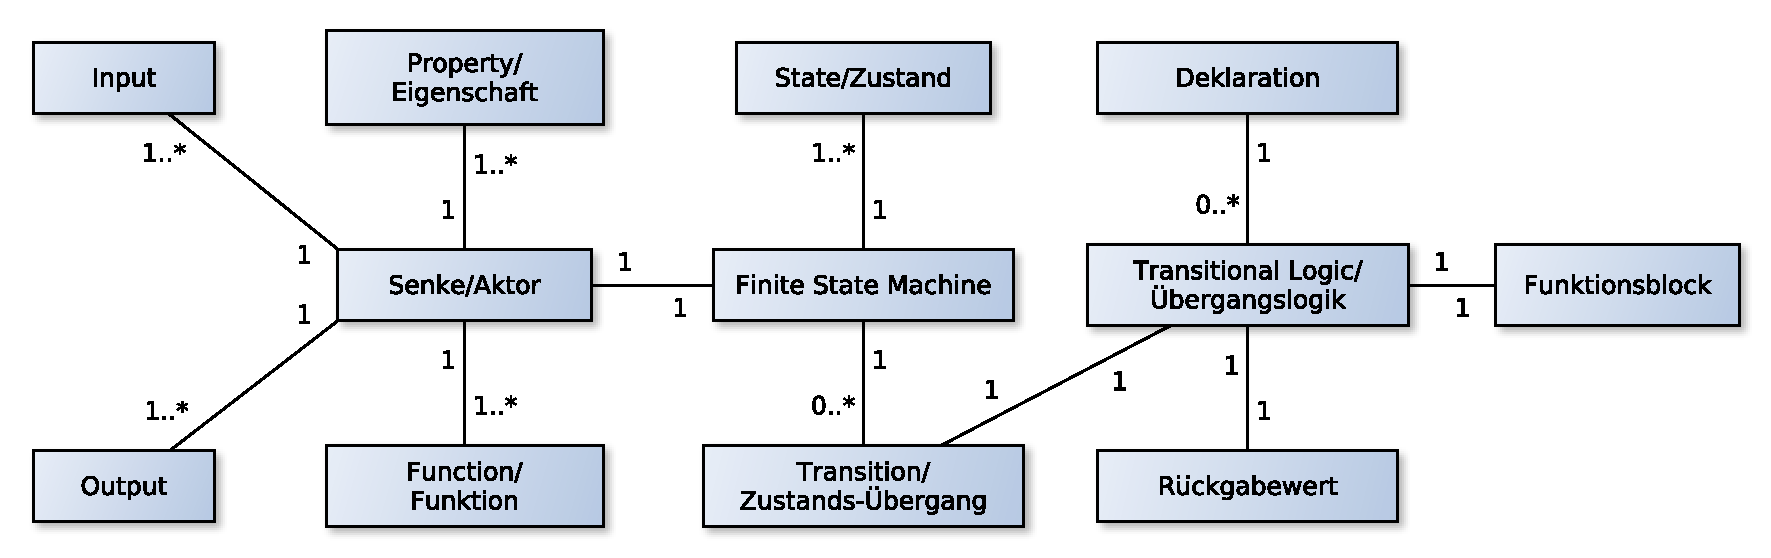
\includegraphics[width=1\textwidth]{bilder/chapter4/chapter4_2/domainmodellaktor.pdf}
  \caption{Das Domänenmodell des Aktors bzw. der \ac{FSM} ist eine Detailansicht von Abbildung \ref{fig:bfddomainmodel} hinsichtlich der Bestandteile des Aktors. }
  \label{fig:domainmodelfsm}
\end{figure}

Durch das Verwenden einer \ac{FSM} ergeben sich mehrere Vorteile. Durch die gute Visualisierung der \ac{FSM} und der weiten Verbreitung des Modells kann die Erlernbarkeit gefördert und somit \hyperref[tab:NFA2]{NFA\#2}, adressiert werden. Zusätzlich erlaubt das Benutzen von \ac{FSM}, wie in  \hyperref[tab:NFA0]{NFA\#0} gefordert, sequentielles Verhalten zu modellieren, indem es die asynchronen Ereignisse, die auf den Aktor-cBlock einwirken, sequentiell zu verarbeiten. Das Hinzufügen von zusätzlichen Aktor-Funktionen durch Experten, kann das System nachträglich erweitert werden, wie es von  \hyperref[tab:NFA5]{NFA\#5} verlangt ist. Im nächsten Schritt muss geklärt werden, wie \ac{DBP} und \ac{FSM} miteinander integriert werden, um Endnutzern das Entwickeln von Programmen innerhalb von flowws zu ermöglichen.